\documentclass[11pt]{beamer}
\usetheme{Madrid}
\usefonttheme{serif}

\usepackage[utf8]{inputenc}
% \usepackage[brazil]{babel}
\usepackage[T1]{fontenc}

\usepackage{amsmath}
\usepackage{amsfonts}
\usepackage{amssymb}
\usepackage{graphicx}

\usepackage{caption}
\usepackage{siunitx}

\usepackage{booktabs}

\DeclareMathOperator{\sen}{sen}
\DeclareMathOperator{\tg}{tg}

\setbeamertemplate{caption}[numbered]

\author[Luna Fonseca]{Luna Fonseca \\ Professor: Hélder Daniel}
\title[Silly Wars]{Silly Wars}
\newcommand{\email}{email}
%\setbeamercovered{transparent} 
\setbeamertemplate{navigation symbols}{} 
\logo{
\includegraphics[scale=0.15]{images/ualg_tiny.png}}
\institute[]{UALG \par MASTERS IN INFORMATICS ENGINEERING} 
\date{16 May, 2025}

% ---------------------------------------------------------
% Selecione um estilo de referência
\bibliographystyle{apalike}

\begin{document}

\begin{frame}
	\titlepage
\end{frame}

\section{Introduction}

\begin{frame}{Introduction}
	\begin{itemize}
		\item RTS (Real-Time Strategy)
		\item Top-down
		\item Tile-based
		\item Match-based
	\end{itemize}
\end{frame}

\section{Units}

\begin{frame}
    \begin{beamercolorbox}[sep=8pt,center,rounded=true,shadow=true]{title}
		\usebeamerfont{title}\Huge\textbf{Units}
    \end{beamercolorbox}
\end{frame}

\begin{frame}{Pawn}
	\begin{columns}
		\begin{column}{0.48\textwidth}
			
\includegraphics[width=\textwidth]{images/pawn.png}
		\end{column}

		\begin{column}{0.48\textwidth}
			\textbf{Stats}
			\begin{itemize}
				\item low hp
				\item low attack
			\end{itemize}
			\textbf{Walking}
			\begin{itemize}
				\item average speed
				\item average sight
			\end{itemize}
			\textbf{Powers}
			\begin{itemize}
				\item can build
				\item can repair structures
				\item can mine
			\end{itemize}
			\textbf{Training}
			\begin{itemize}
				\item average time to train
				\item low cost
			\end{itemize}
		\end{column}
	\end{columns}
\end{frame}

\begin{frame}{Knight}
	\begin{columns}
		\begin{column}{0.48\textwidth}
			
\includegraphics[width=\textwidth]{images/knight.png}
		\end{column}

		\begin{column}{0.48\textwidth}
			\textbf{Stats}
			\begin{itemize}
				\item high hp
				\item medium attack
			\end{itemize}
			\textbf{Walking}
			\begin{itemize}
				\item slow speed
				\item small sight
			\end{itemize}
			\textbf{Powers}
			\begin{itemize}
				\item (none)
			\end{itemize}
			\textbf{Training}
			\begin{itemize}
				\item long time to train
				\item high cost
			\end{itemize}
		\end{column}
	\end{columns}
\end{frame}

\section{Structures}

\begin{frame}
    \begin{beamercolorbox}[sep=8pt,center,rounded=true,shadow=true]{title}
		\usebeamerfont{title}\Huge\textbf{Structures}
    \end{beamercolorbox}
\end{frame}

\begin{frame}{Castle}
	\begin{columns}
		\begin{column}{0.48\textwidth}
			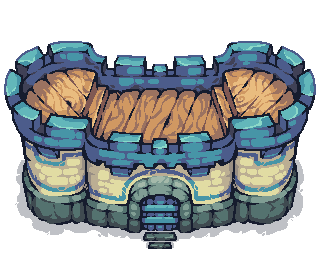
\includegraphics[width=\textwidth]{images/castle.png}
		\end{column}

		\begin{column}{0.48\textwidth}
			\textbf{Stats}
			\begin{itemize}
				\item very high hp
				\item no attack
			\end{itemize}
			\textbf{Effects}
			\begin{itemize}
				\item large sight
			\end{itemize}
			\textbf{Powers}
			\begin{itemize}
				\item generating pawns
			\end{itemize}
			\textbf{Construction}
			\begin{itemize}
				\item long time to build
				\item high cost
			\end{itemize}
		\end{column}
	\end{columns}
\end{frame}

\begin{frame}{Barracks}
	\begin{columns}
		\begin{column}{0.48\textwidth}
			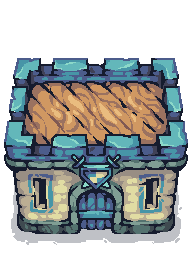
\includegraphics[width=\textwidth]{images/barracks.png}
		\end{column}

		\begin{column}{0.48\textwidth}
			\textbf{Stats}
			\begin{itemize}
				\item low hp
				\item no attack
			\end{itemize}
			\textbf{Effects}
			\begin{itemize}
				\item medium sight
			\end{itemize}
			\textbf{Powers}
			\begin{itemize}
				\item generating knights
			\end{itemize}
			\textbf{Construction}
			\begin{itemize}
				\item medium time to build
				\item medium cost
			\end{itemize}
		\end{column}
	\end{columns}
\end{frame}

\section{Resources}

\begin{frame}
    \begin{beamercolorbox}[sep=8pt,center,rounded=true,shadow=true]{title}
		\usebeamerfont{title}\Huge\textbf{Resources}
    \end{beamercolorbox}
\end{frame}

\begin{frame}{Gold}
	\begin{columns}
		\begin{column}{0.48\textwidth}
			
\includegraphics[width=\textwidth]{images/gold.png}
		\end{column}

		\begin{column}{0.48\textwidth}
			\begin{itemize}
				\item can be depleted
				\item static (immovable)
				\item used for pawns to generate money
				\item maximum of 5 pawns per node
			\end{itemize}
		\end{column}
	\end{columns}
\end{frame}

\section{Mockup}

\begin{frame}
    \begin{beamercolorbox}[sep=8pt,center,rounded=true,shadow=true]{title}
		\usebeamerfont{title}\Huge\textbf{Mockup}
    \end{beamercolorbox}
\end{frame}

\begin{frame}{Whole Map}
	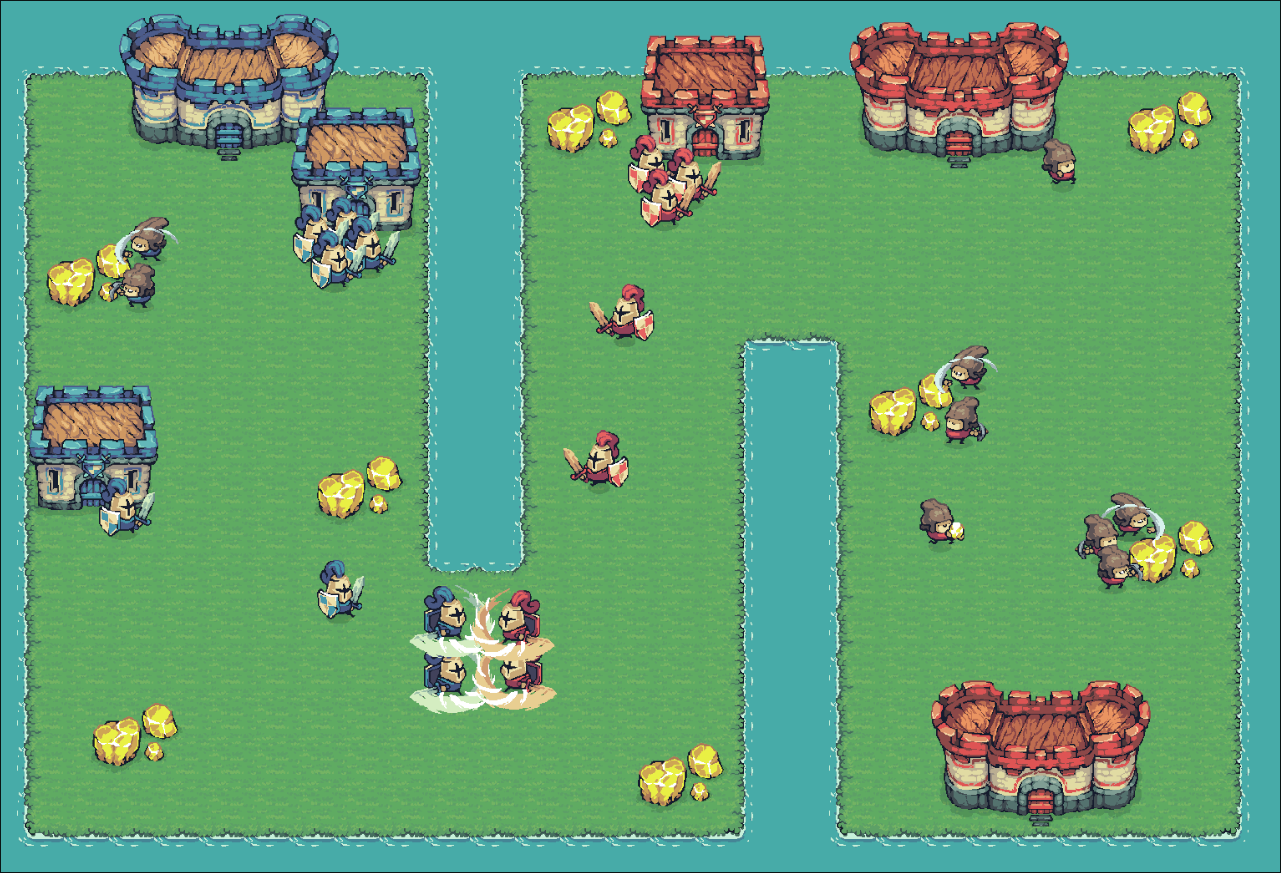
\includegraphics[width=\textwidth]{images/map.png}
\end{frame}

\begin{frame}{Fog}
	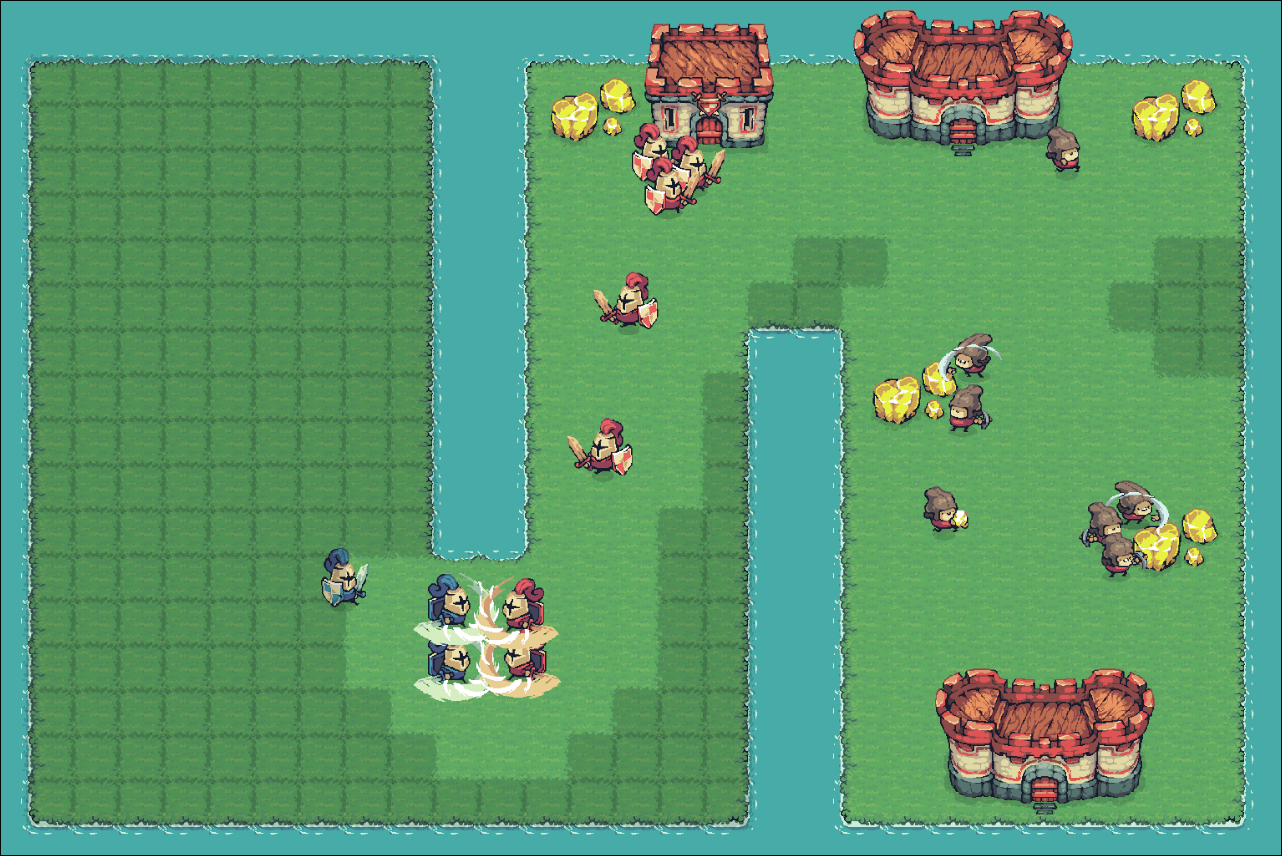
\includegraphics[width=\textwidth]{images/fog.png}
\end{frame}

\begin{frame}{Pawn UI}
	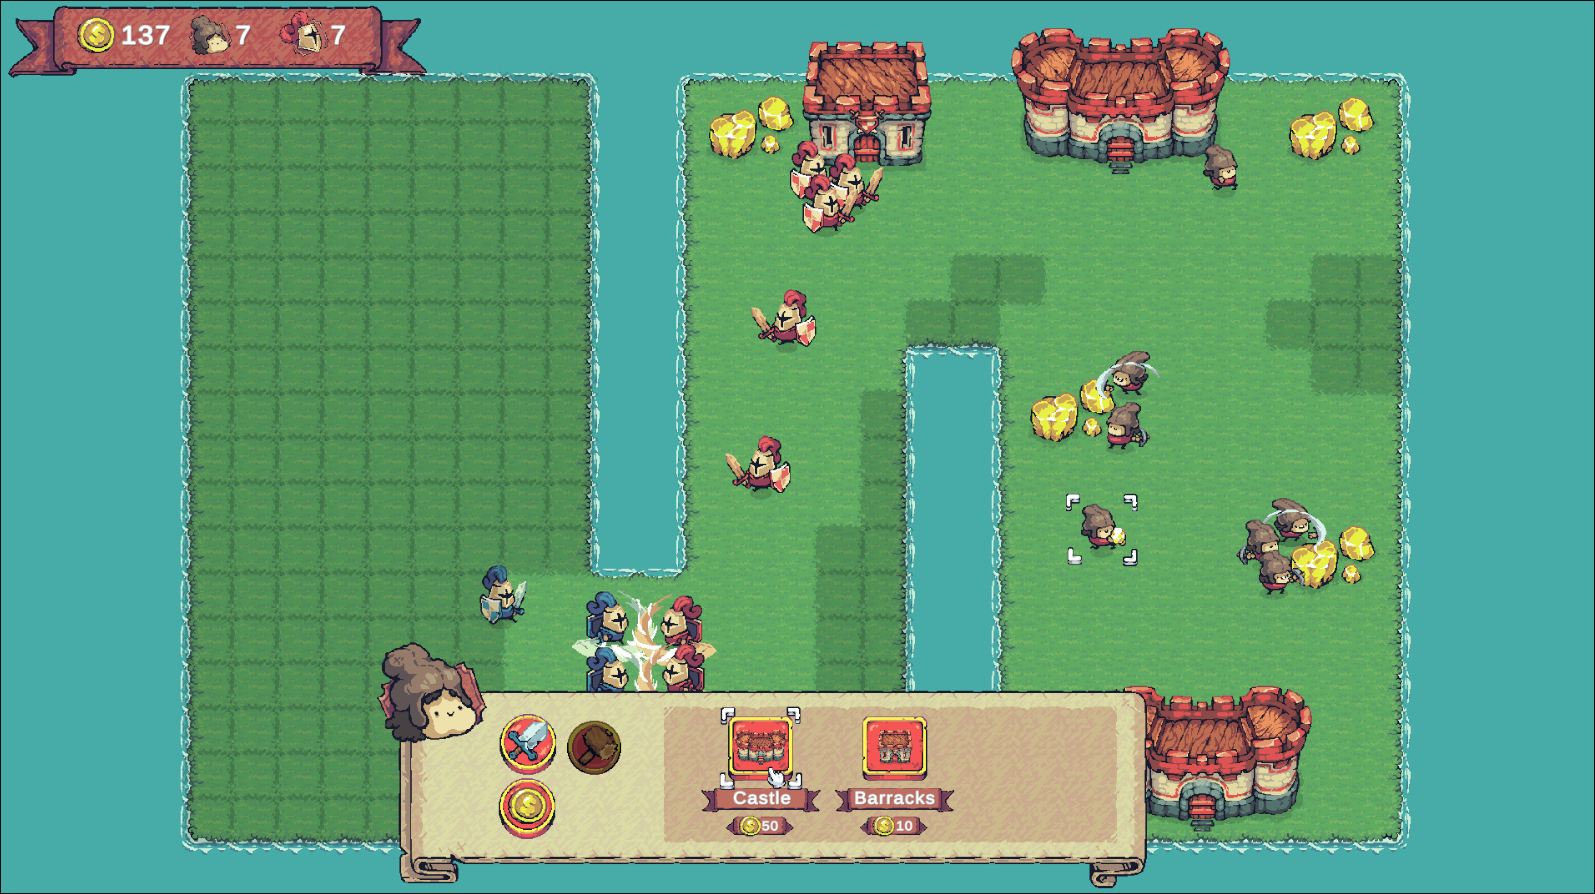
\includegraphics[width=\textwidth]{images/ui_pawn.png}
\end{frame}

\begin{frame}{Knight UI}
	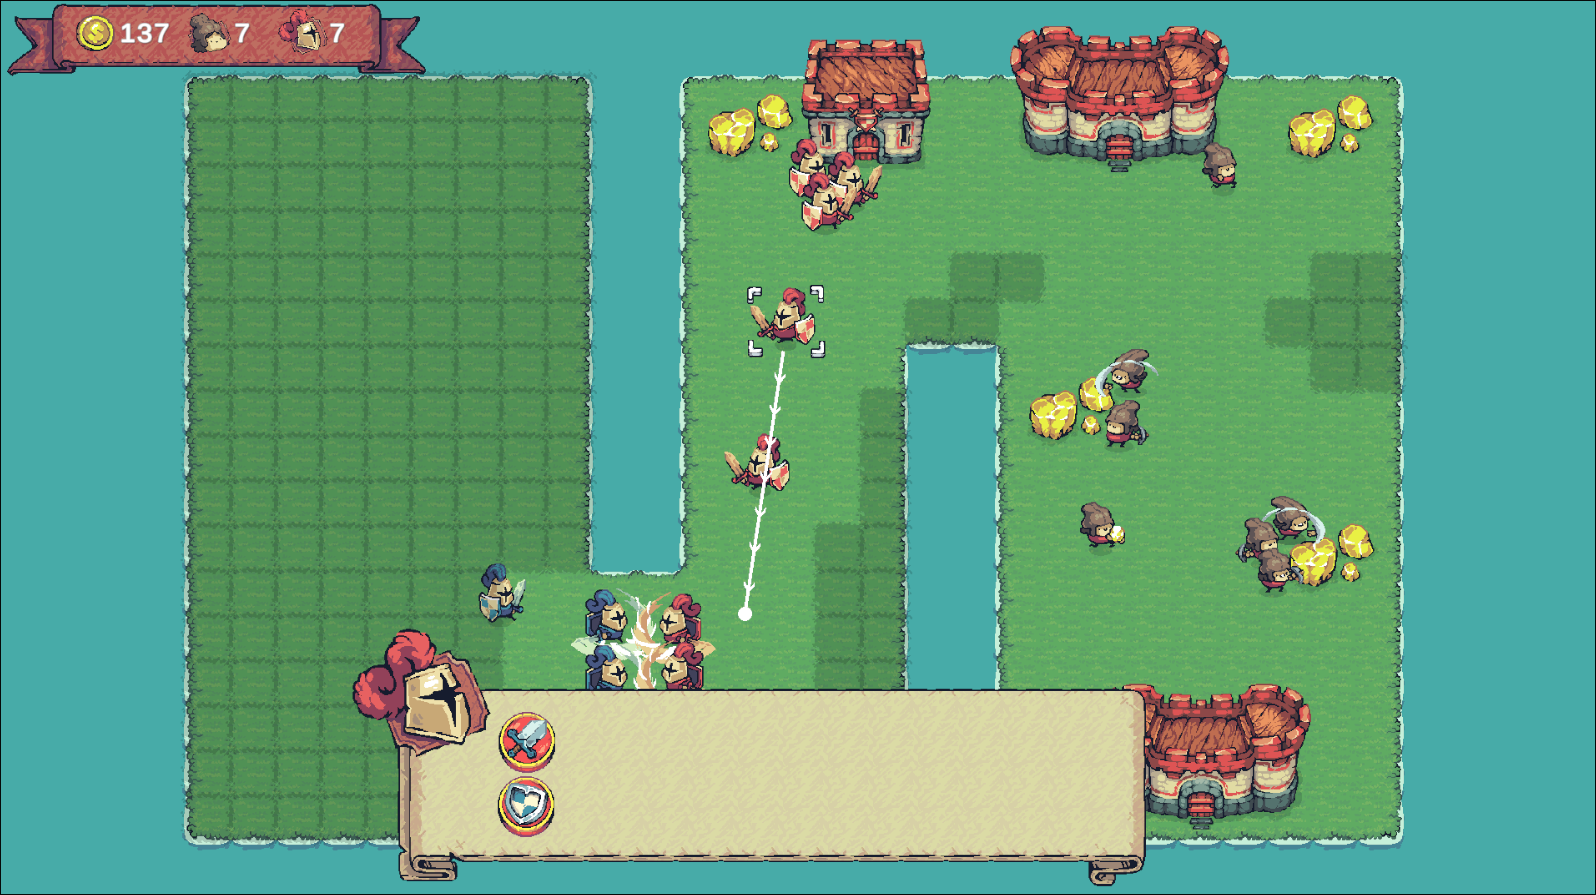
\includegraphics[width=\textwidth]{images/ui_knight.png}
\end{frame}

\end{document}
